\documentclass[letterpaper,twocolumn,10pt]{article}
\usepackage{usenix-2020-09}

\usepackage{amsmath}
\usepackage{booktabs}
\usepackage{enumitem}
\usepackage{graphicx}
\usepackage{multirow}
\usepackage{tikz}
\usetikzlibrary{arrows.meta,positioning}

\newcommand{\sys}{RDMA Cache Prototype}
\newcommand{\todo}[1]{}

%-------------------------------------------------------------------------------
\begin{document}
%-------------------------------------------------------------------------------

\date{}

\title{\Large \bf Evaluating RDMA for Distributed Cache Reads and Metadata Updates}

\author{
{\rm Aengus McGuinness}\\
CS2640 Final Project
}

\maketitle

%-------------------------------------------------------------------------------
\begin{abstract}
%-------------------------------------------------------------------------------
Distributed caches improve application latency by serving hot objects from
memory, but every cache access still incurs server CPU work and often updates
eviction metadata.  This project asks how much of that overhead can be removed
with Remote Direct Memory Access (RDMA), and how much of the benefit remains
when read operations also perform lightweight metadata updates.  I built
\sys{}, a minimal key-value cache with three communication paths: a TCP/RPC
baseline, a two-sided RDMA send/receive path, and a one-sided RDMA read path
over a remotely readable hash table.  The one-sided path can optionally issue
an RDMA \texttt{FETCH\_AND\_ADD} after each read to approximate LRU-style
recency metadata maintenance.  In a final three-trial CloudLab experiment,
two-sided RDMA improves throughput by 5.5--13.2$\times$ over TCP and reduces
p99 latency from 132--164~$\mu$s to 6--8~$\mu$s.  One-sided reads reach
160k--974k operations/s with stable 12~$\mu$s p99 latency.  Metadata atomics
increase one-sided mean latency by about 3.0--3.2~$\mu$s and p99 latency by
3--4~$\mu$s.  These results show that one-sided RDMA can remove most
server-side cache read overhead, but metadata maintenance remains a visible
part of the critical path.
\end{abstract}

%-------------------------------------------------------------------------------
\section{Introduction}
%-------------------------------------------------------------------------------

Distributed caching systems such as Memcached, Redis, and Valkey are a common
way to reduce database load and improve tail latency.  They are simple in
concept: clients send key-value requests to a cache server, and the server
returns values from memory.  At high request rates, however, even simple cache
reads are not free.  Each request enters the server through the operating
system network stack, wakes application code, parses a command, performs a
lookup, formats a response, and sends data back to the client.  A read may
also update eviction metadata, such as an LRU order or access counter.

RDMA changes this design space.  With one-sided RDMA, a client can read or
write registered memory on a remote machine without involving the remote CPU.
If cache objects are laid out so clients can compute where values live, then
cache reads can bypass the server's request-processing loop entirely.  The
main complication is metadata. Practical caches rarely perform pure reads, since
they also track object recency, frequency, or admission information.  These
metadata updates can reintroduce remote communication and synchronization.

This project evaluates that trade-off with a small but working prototype.
The original proposal defined three goals.  The 75\% goal was to implement a
basic key-value store and compare TCP/RPC to two-sided RDMA messaging.  The
100\% goal was to add one-sided RDMA reads.  The 125\% goal was to simulate
cache metadata updates and measure their impact on one-sided RDMA.  \sys{}
implements all three configurations and collects throughput, latency, server
CPU, and attempted network-counter measurements on CloudLab.

This report makes three contributions:
\begin{itemize}[leftmargin=*,noitemsep]
\item It implements a common key-value workload across TCP, two-sided RDMA,
and one-sided RDMA, while preserving comparable request semantics where the
transport allows it.
\item It defines a fixed RDMA-readable hash table layout that lets clients
issue one-sided reads without server CPU participation.
\item It measures the latency cost of adding RDMA atomic metadata updates to
the one-sided read path.
\end{itemize}

Overall, the results show that RDMA reduces cache-read overhead, while metadata updates remain a visible cost.


%-------------------------------------------------------------------------------
\section{Background and Goals}
%-------------------------------------------------------------------------------

\subsection{Communication Modes}

\textbf{TCP/RPC.}
The baseline follows the usual client-server model.  Clients send textual
\texttt{GET}, \texttt{SET}, \texttt{DEL}, and \texttt{QUIT} commands over TCP.
The server parses each request, calls a local key-value store, and sends a
text response.  This mode represents the traditional RPC-style distributed
cache structure.

\textbf{Two-sided RDMA.}
Two-sided RDMA still involves both machines: the client posts an RDMA
\texttt{SEND}, and the server must have posted a matching \texttt{RECV}.  The
server CPU still parses and handles each request, but the transport bypasses
the normal TCP socket data path.  This isolates the benefit of RDMA messaging.

\textbf{One-sided RDMA.}
One-sided RDMA lets the client issue an RDMA \texttt{READ} directly against
the server's registered memory.  Once the queue pair and memory region are
established, the data path does not require server CPU execution.  This mode
matches the central read-heavy cache optimization from the proposal.

\subsection{Metadata Updates}

The difficult part of one-sided caching is not fetching bytes; it is preserving
cache policy.  LRU-like policies update metadata on every access.  A complete
distributed LRU list would require ordering, synchronization, and consistency
protocols.  For this project, I use a narrower but measurable proxy: each
cache slot contains an 8-byte \texttt{access\_count}.  The metadata variant of
the one-sided benchmark performs one RDMA \texttt{FETCH\_AND\_ADD} after each
RDMA read.  This does not implement full LRU, but it captures the essential
cost that every read must also modify remote metadata.

%-------------------------------------------------------------------------------
\section{Design}
%-------------------------------------------------------------------------------

\subsection{System Overview}

\sys{} is organized into storage, protocol, transport, and benchmark layers.
The TCP and two-sided RDMA modes use the same text protocol and same
\texttt{KeyValueStore} logic.  The one-sided mode uses a different storage
layout because remote clients need deterministic address arithmetic.

\begin{figure*}[t]
\centering
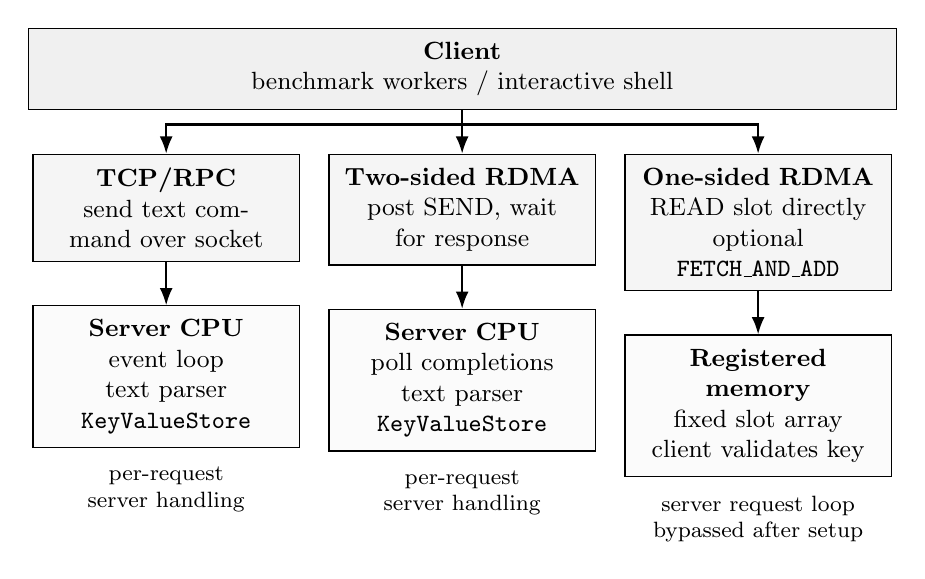
\begin{tikzpicture}[
  font=\small,
  box/.style={draw, align=center, inner sep=5pt, minimum height=0.7cm},
  mode/.style={box, fill=gray!8, text width=0.25\textwidth},
  work/.style={box, fill=gray!3, text width=0.25\textwidth},
  note/.style={align=center, text width=0.25\textwidth, font=\footnotesize},
  arrow/.style={-{Latex[length=2.2mm]}, thick}
]
\node[box, fill=gray!12, text width=0.88\textwidth] (client)
  {\textbf{Client}\\benchmark workers / interactive shell};

\node[mode, below=0.55cm of client.south, anchor=north, xshift=-0.31\textwidth] (tcp)
  {\textbf{TCP/RPC}\\send text command over socket};
\node[mode, below=0.55cm of client.south, anchor=north] (rdma2)
  {\textbf{Two-sided RDMA}\\post SEND, wait for response};
\node[mode, below=0.55cm of client.south, anchor=north, xshift=0.31\textwidth] (rdma1)
  {\textbf{One-sided RDMA}\\READ slot directly\\optional \texttt{FETCH\_AND\_ADD}};

\node[work, below=0.55cm of tcp] (tcpwork)
  {\textbf{Server CPU}\\event loop\\text parser\\\texttt{KeyValueStore}};
\node[work, below=0.55cm of rdma2] (rdma2work)
  {\textbf{Server CPU}\\poll completions\\text parser\\\texttt{KeyValueStore}};
\node[work, below=0.55cm of rdma1] (rdma1work)
  {\textbf{Registered memory}\\fixed slot array\\client validates key};

\node[note, below=0.12cm of tcpwork] {per-request server handling};
\node[note, below=0.12cm of rdma2work] {per-request server handling};
\node[note, below=0.12cm of rdma1work] {server request loop bypassed after setup};

\draw[arrow] (client.south) -- ++(0,-0.18) -| (tcp.north);
\draw[arrow] (client.south) -- (rdma2.north);
\draw[arrow] (client.south) -- ++(0,-0.18) -| (rdma1.north);
\draw[arrow] (tcp.south) -- (tcpwork.north);
\draw[arrow] (rdma2.south) -- (rdma2work.north);
\draw[arrow] (rdma1.south) -- (rdma1work.north);
\end{tikzpicture}
\caption{Data paths compared in \sys{}.  TCP and two-sided RDMA both execute
server-side request handling on every operation.  One-sided RDMA reads the
registered slot array directly, optionally issuing one atomic metadata update,
and bypasses the server request loop after connection setup.}
\label{fig:architecture}
\end{figure*}

\subsection{TCP Baseline}

The TCP server uses a single-threaded coroutine event loop built on
\texttt{poll(2)}.  It accepts multiple client connections, sets sockets to
nonblocking mode, buffers partial reads and writes, and resumes connection
coroutines when descriptors become ready.  The store is a
\texttt{std::unordered\_map} protected by a mutex.  This implementation is
small, but it avoids a thread-per-connection design that would make the TCP
baseline less comparable to a high-performance network server.

\subsection{Two-Sided RDMA}

The RDMA transport is implemented using \texttt{libibverbs}.  Each connection
owns a Reliable Connected queue pair, a completion queue, a protection domain,
and pinned send/receive buffers.  A TCP side channel exchanges queue-pair
metadata: QP number, LID, GID, and, in one-sided mode, the remote key and base
address of the exported memory region.  After the exchange, the code moves the
queue pair through \texttt{INIT}, \texttt{RTR}, and \texttt{RTS}.  The
two-sided server then repeatedly receives text requests, runs the same protocol
handler used by TCP, and sends text responses.

\subsection{One-Sided Memory Layout}

One-sided reads require the client to know where a key may reside without
asking the server.  The one-sided store is therefore a flat open-addressing
hash table with 4096 fixed-size slots.  Each slot is exactly 1024 bytes and is
aligned to 1024 bytes.  The full registered region is 4~MiB.

\begin{table}[h!]
\centering
\caption{RDMA-readable slot layout.}
\label{tab:slot-layout}
\begin{tabular}{rll}
\toprule
Offset & Size & Field \\
\midrule
0   & 1 B   & \texttt{occupied} state \\
1   & 7 B   & padding \\
8   & 8 B   & \texttt{access\_count} metadata \\
16  & 112 B & null-terminated key \\
128 & 896 B & null-terminated value \\
\midrule
Total & 1024 B & one \texttt{RdmaSlot} \\
\bottomrule
\end{tabular}
\end{table}

The client replicates the server's FNV-1a hash function and linear-probing
logic.  For a \texttt{GET}, it computes the initial slot index, issues an RDMA
read for the slot, checks the occupied byte and key, and continues probing if
necessary.  The metadata path then issues an RDMA \texttt{FETCH\_AND\_ADD} to
the slot's \texttt{access\_count} field at offset 8.  That offset satisfies
the 8-byte alignment required for Mellanox atomics.

\subsection{Benchmark and Automation}

The project includes two benchmark executables.  \texttt{kv\_benchmark}
targets the TCP server.  \texttt{kv\_client\_rdma --benchmark} performs the
required RDMA handshake and then runs the same style of workload against the
RDMA modes.  Both emit CSV files with elapsed time, throughput, mean latency,
p50, p95, p99, and error counts.  Runner scripts execute the TCP, two-sided
RDMA, and one-sided RDMA sweeps on CloudLab and regenerate plots locally.

%-------------------------------------------------------------------------------
\section{Experimental Methodology}
%-------------------------------------------------------------------------------

\subsection{Environment}

Experiments were run on a two-node CloudLab setup with RDMA-capable Mellanox
hardware.  The server and client communicated over the private 10.10.x.x
experiment network.  A device-mapping check showed that the private experiment
interface was \texttt{ens1f1np1}, backed by RDMA device \texttt{mlx5\_3}; the
public/control interface was \texttt{eno49np0}, backed by \texttt{mlx5\_0}.
All final RDMA measurements therefore used \texttt{--device mlx5\_3} and
sampled \texttt{ens1f1np1} for host network counters.  The code was built with
CMake and \texttt{libibverbs}; RDMA targets are compiled only when the verbs
library is available.

\begin{table}[h!]
\centering
\caption{Final CloudLab experiment configuration.}
\label{tab:environment}
\begin{tabular}{ll}
\toprule
Item & Value \\
\midrule
Server data IP & \texttt{10.10.1.1} \\
Client data IP & \texttt{10.10.1.2} \\
Private netdev & \texttt{ens1f1np1} \\
RDMA device & \texttt{mlx5\_3} \\
Control netdev & \texttt{eno49np0} \\
Control RDMA device & \texttt{mlx5\_0} \\
Compiler & GNU C++ 11.4.0 \\
Build system & CMake + \texttt{libibverbs} \\
Trials per point & 3 \\
\bottomrule
\end{tabular}
\end{table}

\subsection{Workloads}

The final client-count sweep used 1, 2, 4, and 8 clients with 100,000 measured
operations per point, 5,000 warmup operations, and 1024 prefilled keys.  Each
point was repeated three times.  TCP and two-sided RDMA used 64-byte values, a
95\% GET ratio, and Zipf skew $s=0.8$.

These parameters were chosen to make the experiment large enough to produce stable measurements while keeping the workload focused on transport overhead. The client counts form a power-of-two scaling sweep from a single-client baseline to modest concurrency.  Each point uses 100,000 measured operations, which reduced variance relative to earlier 10,000-operation runs, and 5,000 warmup operations to exclude connection setup, queue initialization, and cold cache effects from the measured interval.  The 1024-key working set is intentionally small and preloaded which keeps the data resident and avoids conflating transport costs with capacity misses, paging, or large hash-table behavior.  The 64-byte value size represents small cache objects, where fixed software and transport overheads are especially important.




Because the one-sided prototype supports
direct reads over a preloaded RDMA slot array, its measurements are GET-only. The
three-way comparison should therefore be read as a cache-read comparison rather
than a complete replacement for mixed GET/SET service.

The metadata experiment compared one-sided reads with and without one
\texttt{FETCH\_AND\_ADD} per operation.  All final runs completed with zero
warmup errors and zero measured errors.

\subsection{Metrics}

Throughput is measured as completed operations divided by timed elapsed time.
Latency is measured on the client side and reported as mean, median, p95, and
p99.  Plots show the mean across three trials with error bars representing
sample standard deviation.  Server process CPU was sampled externally so the
benchmark hot paths did not include instrumentation.

I also attempted server NIC byte-counter measurements after correcting the
RDMA device mapping to \texttt{mlx5\_3}/\texttt{ens1f1np1}.  TCP counter
values were plausible, but RDMA still reported near-zero bytes per operation.

%-------------------------------------------------------------------------------
\section{Results}
%-------------------------------------------------------------------------------

\subsection{Transport Comparison}

Figure~\ref{fig:transport-comparison} shows the main comparison across TCP,
two-sided RDMA, and one-sided RDMA.  TCP scales from 8.9k operations/s at one
client to 72.9k operations/s at eight clients.  Two-sided RDMA reaches 117k
operations/s at one client and 404k operations/s at eight clients, a
5.5--13.2$\times$ improvement over TCP depending on concurrency.  One-sided
RDMA reads reach 161k operations/s at one client and 974k operations/s at
eight clients.

\begin{figure*}[t]
\centering
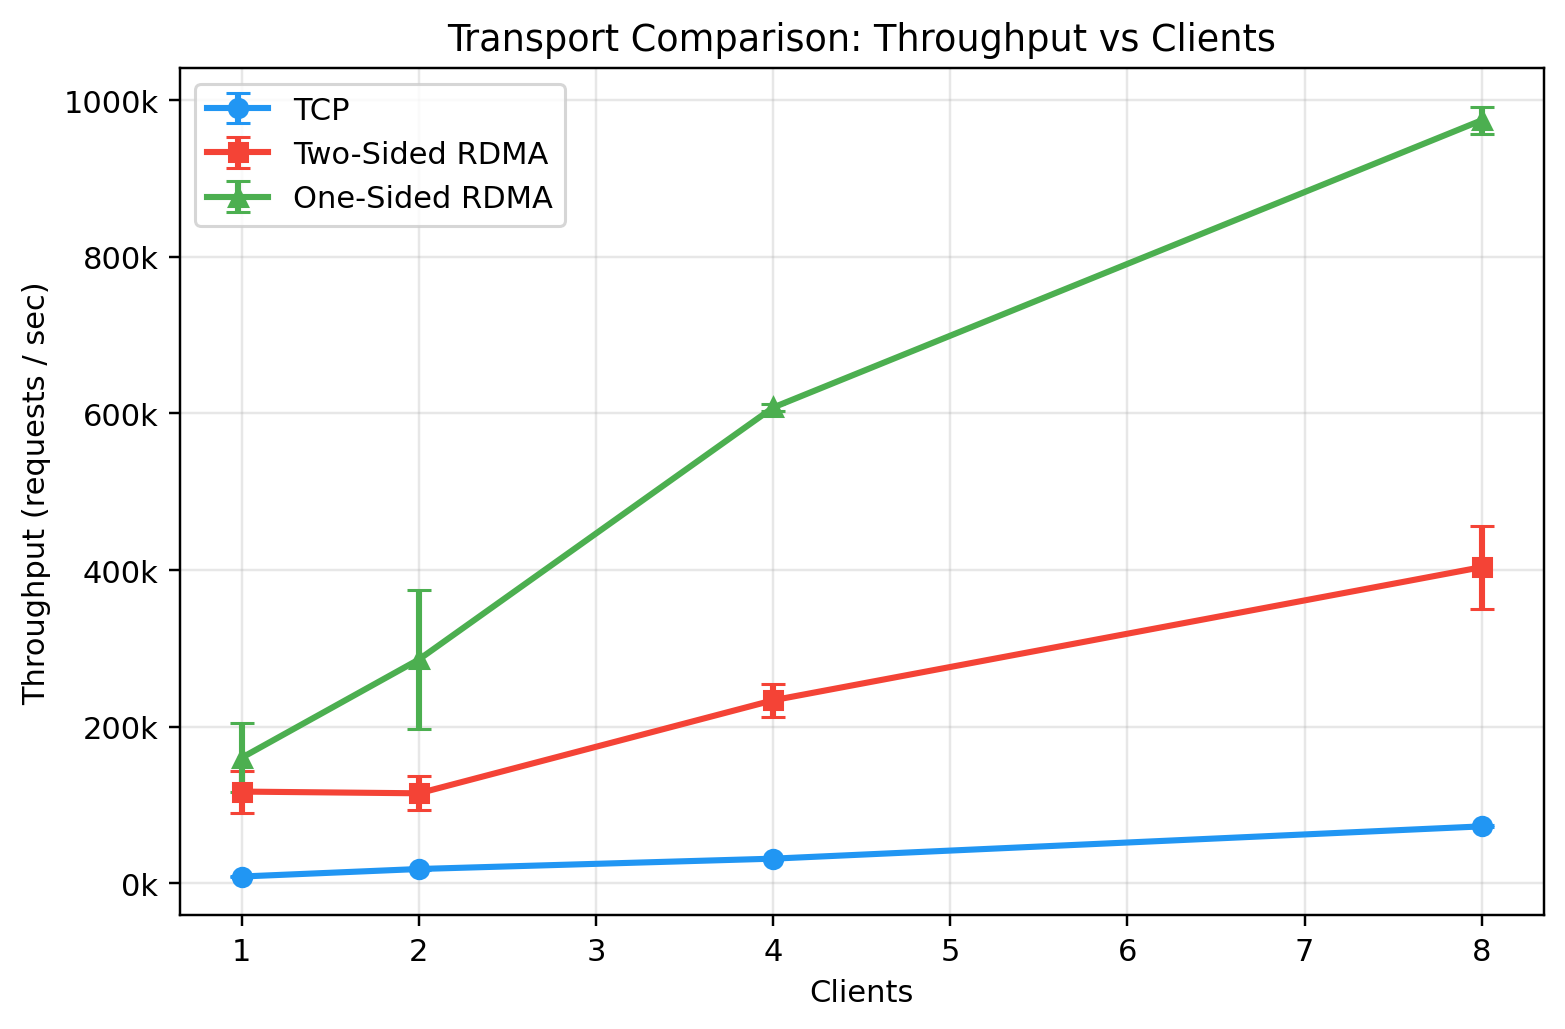
\includegraphics[width=0.49\textwidth]{plots/final_summary_mlx5_3_100k/comparison/throughput_vs_clients_errorbars.png}
\hfill
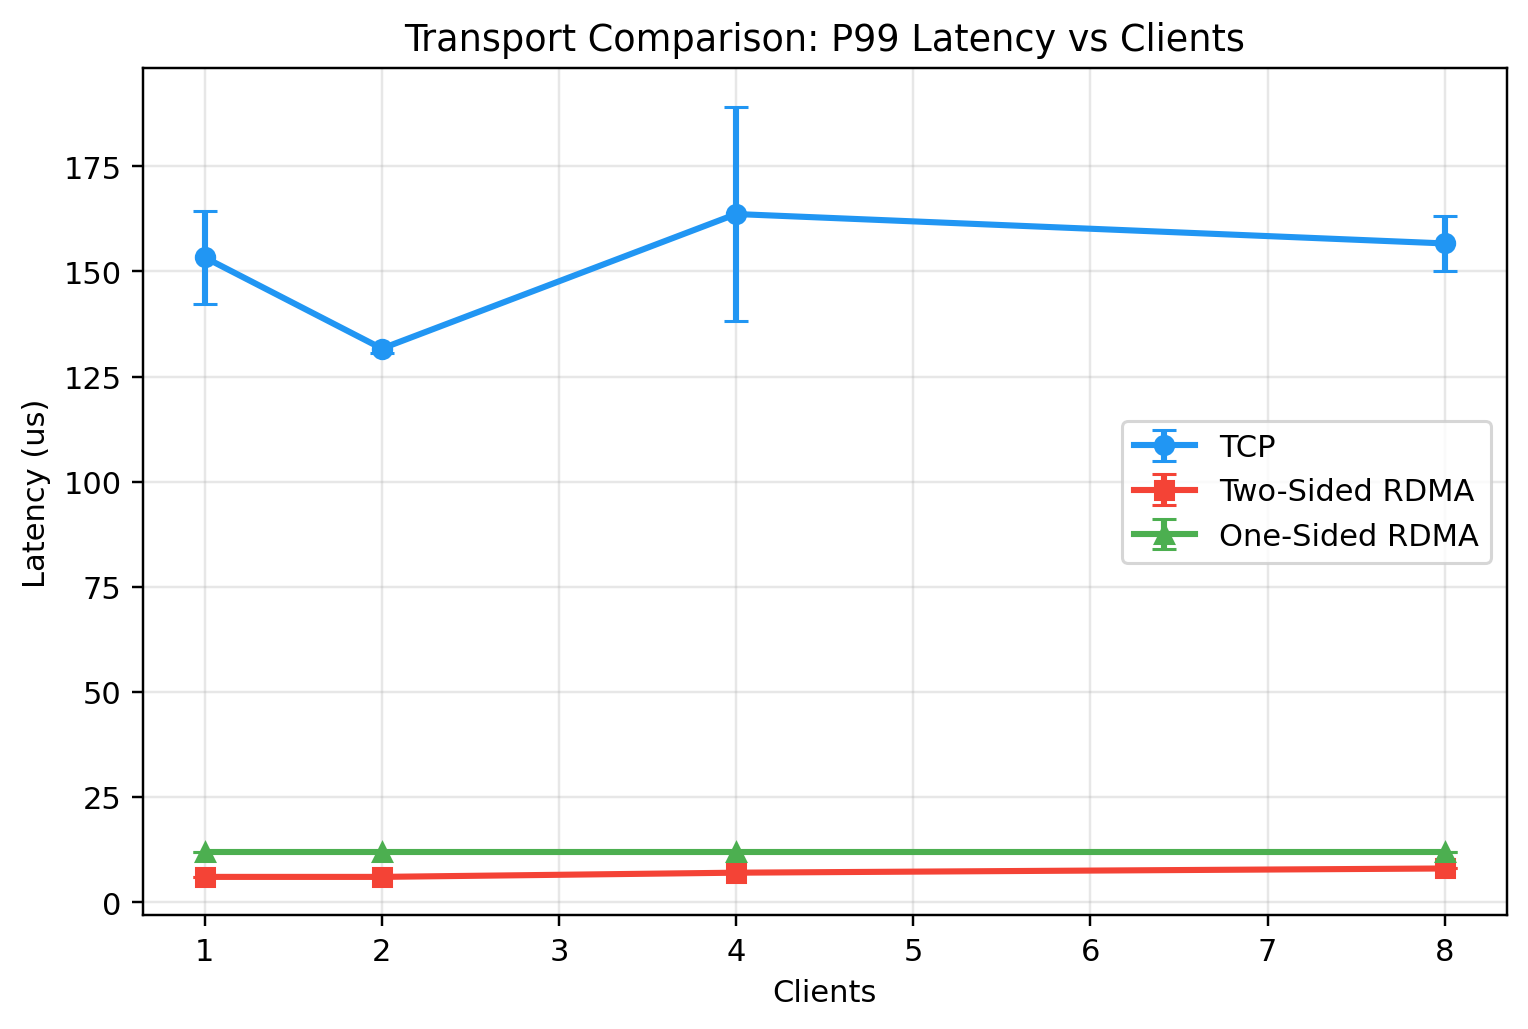
\includegraphics[width=0.49\textwidth]{plots/final_summary_mlx5_3_100k/comparison/p99_latency_vs_clients_errorbars.png}
\caption{Transport comparison on CloudLab.  Points are means across three
trials and error bars show sample standard deviation.  Two-sided RDMA
substantially improves throughput over TCP while keeping server-side request
processing.  One-sided RDMA directly reads registered memory and provides the
lowest read latency, but this sweep is GET-only and should be interpreted as
the direct cache-read path.}
\label{fig:transport-comparison}
\end{figure*}

The p99 latency results are more dramatic.  TCP p99 latency is 132--164
$\mu$s across the sweep.  Two-sided RDMA reduces p99 latency to 6--8
$\mu$s.  One-sided RDMA reports a stable 12~$\mu$s p99 latency at every
client count.  These results support the first two proposal goals: RDMA
messaging improves significantly on TCP, and one-sided reads remove most of
the remaining server-side request overhead.

\begin{table*}[t]
\centering
\caption{Primary client-count results, averaged across three trials.
Throughput is in thousands of operations per second.  All runs reported zero
measured errors.}
\label{tab:primary-results}
\begin{tabular}{llrrrr}
\toprule
Mode & Workload & Clients & Throughput & Mean latency & p99 latency \\
     &          &         & (kops/s)   & ($\mu$s)     & ($\mu$s) \\
\midrule
\multirow{4}{*}{TCP} & 95\% GET, Zipf 0.8 & 1 & 8.9  & 106.4 & 153 \\
                     &                     & 2 & 18.5 & 100.3 & 132 \\
                     &                     & 4 & 31.7 & 110.9 & 164 \\
                     &                     & 8 & 72.9 & 95.3  & 157 \\
\midrule
\multirow{4}{*}{Two-sided RDMA} & 95\% GET, Zipf 0.8 & 1 & 117.3 & 6.2  & 6 \\
                                &                     & 2 & 115.1 & 11.2 & 6 \\
                                &                     & 4 & 233.9 & 13.7 & 7 \\
                                &                     & 8 & 403.8 & 15.2 & 8 \\
\midrule
\multirow{4}{*}{One-sided RDMA} & GET-only reads & 1 & 160.5 & 4.8 & 12 \\
                                &                & 2 & 285.9 & 4.8 & 12 \\
                                &                & 4 & 607.6 & 4.8 & 12 \\
                                &                & 8 & 974.3 & 4.8 & 12 \\
\bottomrule
\end{tabular}
\end{table*}

\subsection{Metadata Overhead}

Figure~\ref{fig:metadata-overhead} isolates the cost of cache metadata
updates.  Adding one RDMA atomic operation after each one-sided read increases
mean latency from roughly 4.8~$\mu$s to 7.8--8.0~$\mu$s.  p99 latency rises
from 12~$\mu$s to 15--16~$\mu$s.

\begin{figure*}[t]
\centering

\includegraphics[width=0.32\textwidth]{plots/final_summary_mlx5_3_100k/metadata_overhead/throughput_vs_clients_errorbars.png}
\hfill

\includegraphics[width=0.32\textwidth]{plots/final_summary_mlx5_3_100k/metadata_overhead/mean_latency_vs_clients_errorbars.png}
\hfill

\includegraphics[width=0.32\textwidth]{plots/final_summary_mlx5_3_100k/metadata_overhead/p99_latency_vs_clients_errorbars.png}
\caption{One-sided RDMA metadata overhead.  The metadata variant performs an
RDMA \texttt{FETCH\_AND\_ADD} after every RDMA read.  Points are means across
three trials and error bars show sample standard deviation.  The atomic
operation reduces throughput and adds a consistent latency penalty, which is
the central cost predicted by the proposal.}
\label{fig:metadata-overhead}
\end{figure*}

The throughput results also show a metadata cost in the final trials.  The
metadata variant is 27--36\% lower throughput than pure one-sided reads across
the client-count sweep.  

\begin{table}[t]
\centering
\caption{Added latency from one RDMA metadata atomic per read.}
\label{tab:metadata-results}
\begin{tabular}{rrrr}
\toprule
Clients & Mean increase & p99 increase & Metadata p99 \\
        & ($\mu$s)      & ($\mu$s)     & ($\mu$s) \\
\midrule
1 & 3.0 & 3.0 & 15.0 \\
2 & 3.1 & 3.7 & 15.7 \\
4 & 3.1 & 4.0 & 16.0 \\
8 & 3.2 & 4.0 & 16.0 \\
\bottomrule
\end{tabular}
\end{table}

\subsection{Server CPU Utilization}

Figure~\ref{fig:cpu} shows sampled server-process CPU utilization.  TCP server
CPU rises with client count, reaching 60.7\% average process CPU at eight
clients.  Two-sided RDMA consumes more sampled server CPU because the server
busy-polls completions and handles every request, reaching 479\% average
process CPU at eight clients.  The one-sided server stays near idle for most
samples because the server is not on the read data path after setup. However, it is important to note that many RDMA benchmark runs are short enough
to produce only one or a few CPU samples.  The qualitative direction is
meaningful, but the exact percentages should not be overfit.

\begin{figure}[t]
\centering
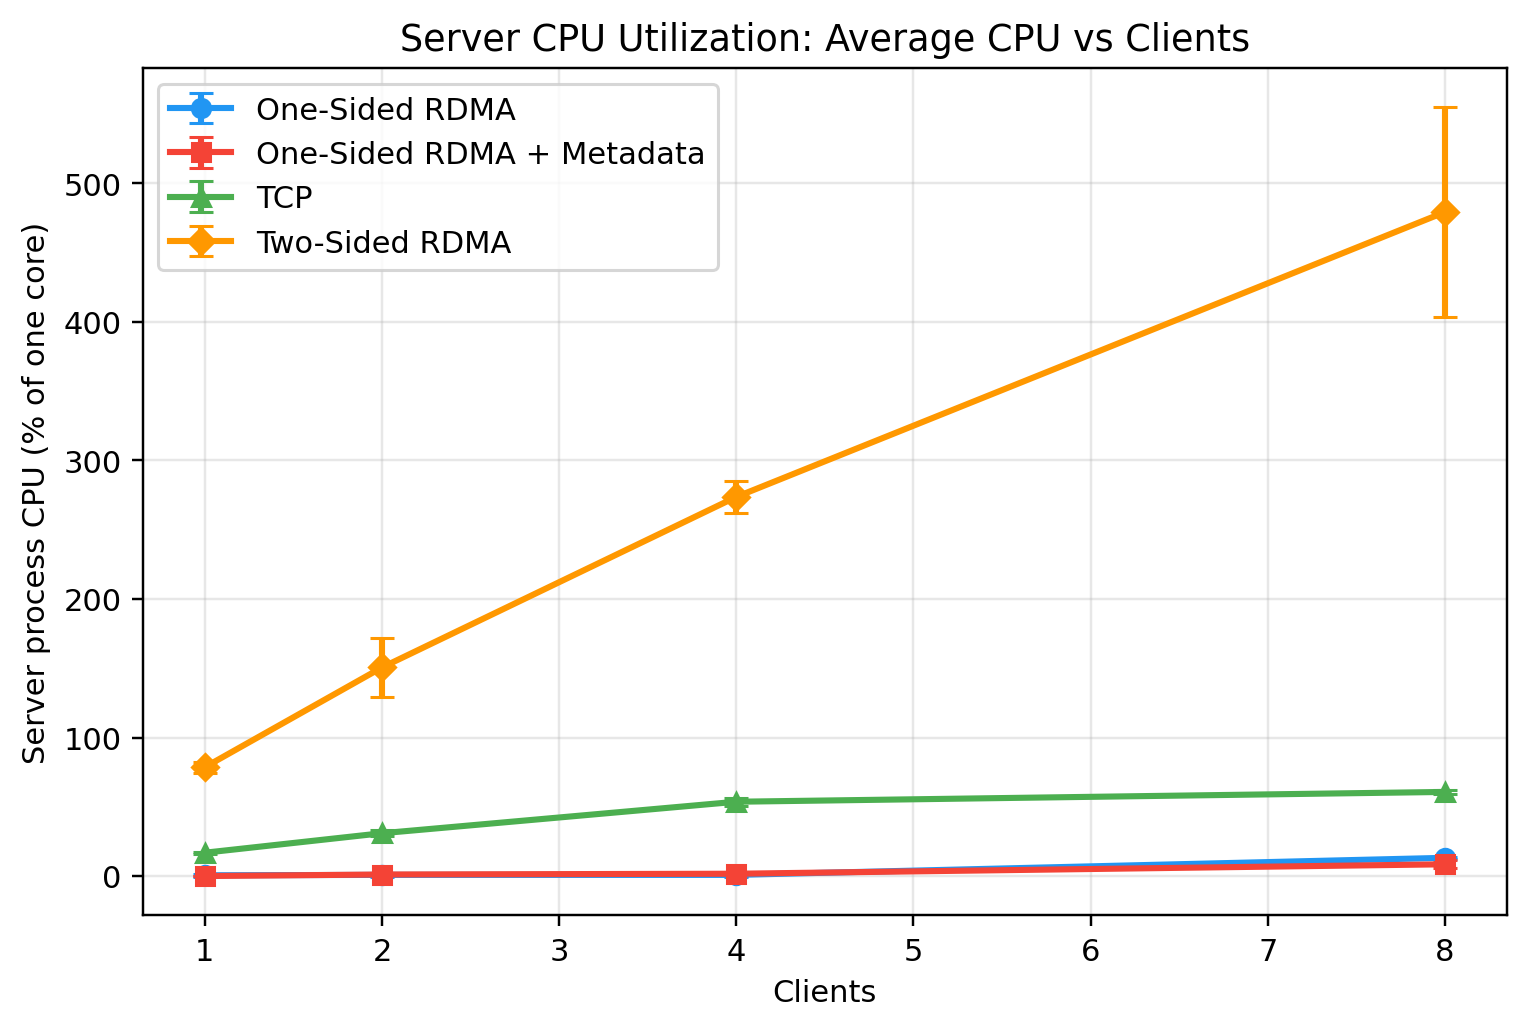
\includegraphics[width=\linewidth]{plots/final_summary_mlx5_3_100k/cpu/avg_server_cpu_vs_clients_errorbars.png}
\caption{Sampled average server-process CPU.  The one-sided server is mostly
idle during the read data path, while TCP and two-sided RDMA require server
CPU work for each request.  Short RDMA runs make this metric noisy.}
\label{fig:cpu}
\end{figure}

\subsection{Network Counter Attempt}

The final automation also recorded server network byte counters on
\texttt{ens1f1np1}.  These measurements are useful mostly as a validation
lesson.  TCP reported a plausible 233 total bytes per operation across all
client counts.  The RDMA modes, however, reported only 0.02--0.08 total bytes
per operation, which is impossible for operations that exchange RDMA messages
or read 1024-byte slots.  I therefore exclude the generated network plot from
the main evidence and treat Linux netdev counters as the wrong instrument for
this RDMA/RoCE traffic on this setup.

%-------------------------------------------------------------------------------
\section{Discussion}
%-------------------------------------------------------------------------------

\subsection{Progress Relative to the Proposal}

The implementation satisfies the proposal's three project tiers.  The 75\%
goal is met by the TCP key-value store, benchmark harness, and two-sided RDMA
comparison.  The 100\% goal is met by the one-sided RDMA read path over a
registered hash-table memory region.  The 125\% goal is substantially met by
the RDMA atomic metadata experiment.  The metadata implementation is not a full
LRU list, but it captures the core issue from the proposal in that every read that
updates cache policy must perform additional remote synchronization.

\subsection{Interpretation}

The results suggest a layered view of RDMA's benefit.  Moving from TCP to
two-sided RDMA removes a large amount of transport overhead but keeps the
server CPU in the critical path.  Moving from two-sided RDMA to one-sided RDMA
removes server request processing from reads, producing very stable read
latency.  Adding metadata atomics then puts a small but consistent remote
synchronization cost back into the path. 

\subsection{Limitations}

The largest experimental limitation is that the one-sided benchmark is
GET-only.  This is appropriate for measuring one-sided reads, but it is not a
complete mixed-operation cache.  The interactive one-sided client supports
RDMA writes, but the benchmark intentionally avoids concurrent one-sided SETs
because a production-quality write protocol would need versioning,
compare-and-swap, or a server-mediated slow path to prevent readers from
observing partially updated slots.

The second limitation is measurement duration.  The final runs use 100,000
operations per point and three trials, which is enough to stabilize the main
latency and throughput trends.  However, the fastest one-sided points still
complete in a fraction of a second, which reduces the reliability of sampled
CPU utilization.  A stronger follow-up experiment would use longer 1M+
operation points for CPU and counter measurements.

Finally, network byte-counter measurements were attempted but are not used as
evidence.  Even after mapping the private experiment network to
\texttt{mlx5\_3}/\texttt{ens1f1np1}, the server's Linux netdev counters
produced plausible TCP bytes per operation but near-zero RDMA bytes per
operation.  This likely means the counter path was not observing the
RoCE/RDMA data path.  Accurate network overhead analysis would need NIC
hardware counters, \texttt{ethtool -S}, \texttt{perfquery}, or
Mellanox-specific RDMA port counters.

%-------------------------------------------------------------------------------
\section{Related Work}
%-------------------------------------------------------------------------------

CliqueMap demonstrated that one-sided RDMA can be used to build production
distributed caching systems, but also showed that the engineering details of
metadata, consistency, and deployment matter greatly~\cite{singhvi21cliquemap}.
Recent work on disaggregated data structures studies the pitfalls of
one-sided RDMA synchronization and emphasizes that avoiding remote CPU work
does not eliminate the need for careful concurrency control~\cite{jasny25rdma}.
Dinomo explores high-performance key-value storage over disaggregated
persistent memory~\cite{lee22dinomo}.  Cache policy work such as lazy
promotion and hit-ratio/throughput studies motivates this project's focus on
metadata: improving hit ratio or recency tracking can hurt throughput when the
metadata path becomes too expensive~\cite{chenLazyPromotion,qiu24hitratio}.

This project is much smaller than those systems, but it targets the same
fundamental trade-off.  By stripping the system down to TCP, two-sided RDMA,
one-sided RDMA, and one metadata atomic, it isolates the cost of each
communication mechanism in a way that is useful for a coarse-grained evaluation.

%-------------------------------------------------------------------------------
\section{Conclusion}
%-------------------------------------------------------------------------------

\sys{} demonstrates that the original proposal was feasible within the project
scope.  The prototype implements a TCP baseline, a two-sided RDMA server, and
a one-sided RDMA read path over a registered hash table.  On CloudLab, RDMA
substantially improves throughput and tail latency relative to TCP.  One-sided
reads achieve low and stable latency without server CPU involvement, while an
RDMA atomic metadata update adds a measurable 3--4~$\mu$s p99 latency cost.

The final answer to the research question is therefore nuanced.  One-sided
RDMA can significantly reduce distributed cache read overhead, but cache
metadata is not free.  Even a simple atomic recency counter consumes part of
the latency budget.  A full production cache would need to decide which
metadata updates truly belong on the read critical path and which can be
batched, approximated, or moved off path.

%-------------------------------------------------------------------------------
\section*{Availability}
%-------------------------------------------------------------------------------

The submitted artifact contains the C++ implementation, CloudLab runner scripts,
raw CSV files, aggregated CSV files, and generated plots. The primary final
inputs are the raw trials under \texttt{experiments/final\_trials\_mlx5\_3\_100k/},
the aggregated CSVs under \texttt{experiments/final\_summary\_mlx5\_3\_100k/},
and the report figures under \texttt{report/plots/final\_summary\_mlx5\_3\_100k/}.

%-------------------------------------------------------------------------------
\begin{thebibliography}{9}

\bibitem{chenLazyPromotion}
Qinghan Chen, Muhammad Haekal Muhyidin, Ziyue Qiu, Zhuofan Chen, Rashmi
Vinayak, and Juncheng Yang.
\newblock Demystifying and Improving Lazy Promotion in Cache Eviction.

\bibitem{jasny25rdma}
Matthias Jasny, Tobias Ziegler, Jacob Nelson-Slivon, Viktor Leis, and Carsten
Binnig.
\newblock Synchronizing disaggregated data structures with one-sided RDMA:
pitfalls, experiments and design guidelines.
\newblock \emph{ACM Transactions on Database Systems}, 50(1), 2025.

\bibitem{lee22dinomo}
Sekwon Lee, Soujanya Ponnapalli, Sharad Singhal, Marcos K. Aguilera, Kimberly
Keeton, and Vijay Chidambaram.
\newblock Dinomo: an elastic, scalable, high-performance key-value store for
disaggregated persistent memory.
\newblock arXiv:2209.08743, 2022.

\bibitem{qiu24hitratio}
Ziyue Qiu, Juncheng Yang, and Mor Harchol-Balter.
\newblock Can Increasing the Hit Ratio Hurt Cache Throughput?
\newblock In \emph{EAI International Conference on Performance Evaluation
Methodologies and Tools}, 2024.

\bibitem{singhvi21cliquemap}
Arjun Singhvi, Aditya Akella, Maggie Anderson, Rob Cauble, Harshad Deshmukh,
Dan Gibson, Milo M. K. Martin, Amanda Strominger, Thomas F. Wenisch, and Amin
Vahdat.
\newblock CliqueMap: productionizing an RMA-based distributed caching system.
\newblock In \emph{Proceedings of ACM SIGCOMM}, 2021.

\end{thebibliography}

%%%%%%%%%%%%%%%%%%%%%%%%%%%%%%%%%%%%%%%%%%%%%%%%%%%%%%%%%%%%%%%%%%%%%%%%%%%%%%%%
\end{document}
%%%%%%%%%%%%%%%%%%%%%%%%%%%%%%%%%%%%%%%%%%%%%%%%%%%%%%%%%%%%%%%%%%%%%%%%%%%%%%%%

%%% Local Variables:
%%% mode: LaTeX
%%% TeX-master: t
%%% End:
